\documentclass[9pt,journal,onecolumn]{IEEEtran}
\usepackage{cite}
\usepackage{amsmath,amssymb,amsfonts}
\usepackage{graphicx}
\usepackage{booktabs}
\usepackage{hyperref}
\usepackage[margin=0.42in]{geometry} % Ultra-tight margins for single-page format
\usepackage{tikz}
\usetikzlibrary{shapes.geometric, arrows, positioning}

\begin{document}

\title{Multi-Fold Multimodal Fusion for Enhanced Cardiovascular Risk Stratification}
\author{Riya Moorjani --- \textit{Precision Clinical Technologies} --- \href{mailto:riyamoorjani2504@gmail.com}{riyamoorjani2504@gmail.com}}
\maketitle
\thispagestyle{empty}
\pagestyle{empty}

\begin{abstract}
Cardiovascular Diseases (CVD) remain the leading cause of global mortality. Classical machine learning (e.g., XGBoost) is restricted to structured tabular features, creating blind spots for acute electrical anomalies, structural lung/heart abnormalities, qualitative narratives, and spatiotemporal motion dynamics. We introduce a secure, multi-fold clinical workstation integrating tabular parameters, 12-lead ECG, chest radiographs, echocardiograms (Echo-analysis), and clinical notes. Utilizing a late-fusion neural adapter, the workstation achieves an accuracy of \textbf{92.1\%}, representing a \textbf{+13.7\% absolute improvement} over the single-modal XGBoost baseline (78.4\%). The system utilizes AES-256 encryption derived from Attending NPI tokens to ensure HIPAA auditing compliance.
\end{abstract}

\section{Introduction \& Rationale}
Traditional clinical risk scores rely solely on structured features. While effective for estimating chronic baselines, these single-modal approaches suffer from major limitations: (1) \textbf{Acute Blind Spots:} Patients may present with normal lab metrics yet experience acute myocardial ischemia visible only on ECG. (2) \textbf{Echocardiography Exclusion:} Valvular stenosis and localized wall motion abnormalities require video spatiotemporal analysis (Echo-analysis) omitted by baseline tabular networks. We propose a \textbf{Multi-Fold Diagnostic Architecture}: Fold 1 acts as a low-compute tabular gate. If Fold 1 detects elevated risk ($\ge 15\%$), it activates Fold 2, extracting deep features from ECG, CXR, Echo, and notes, fusing them into a unified diagnostic index.

\section{System Architecture \& Flowchart}
The workstation operates as a sequential decision gateway. Vitals are scanned in Fold 1, and high-compute unstructured streams are activated in Fold 2 when triggered.

\begin{figure}[h]
\centering
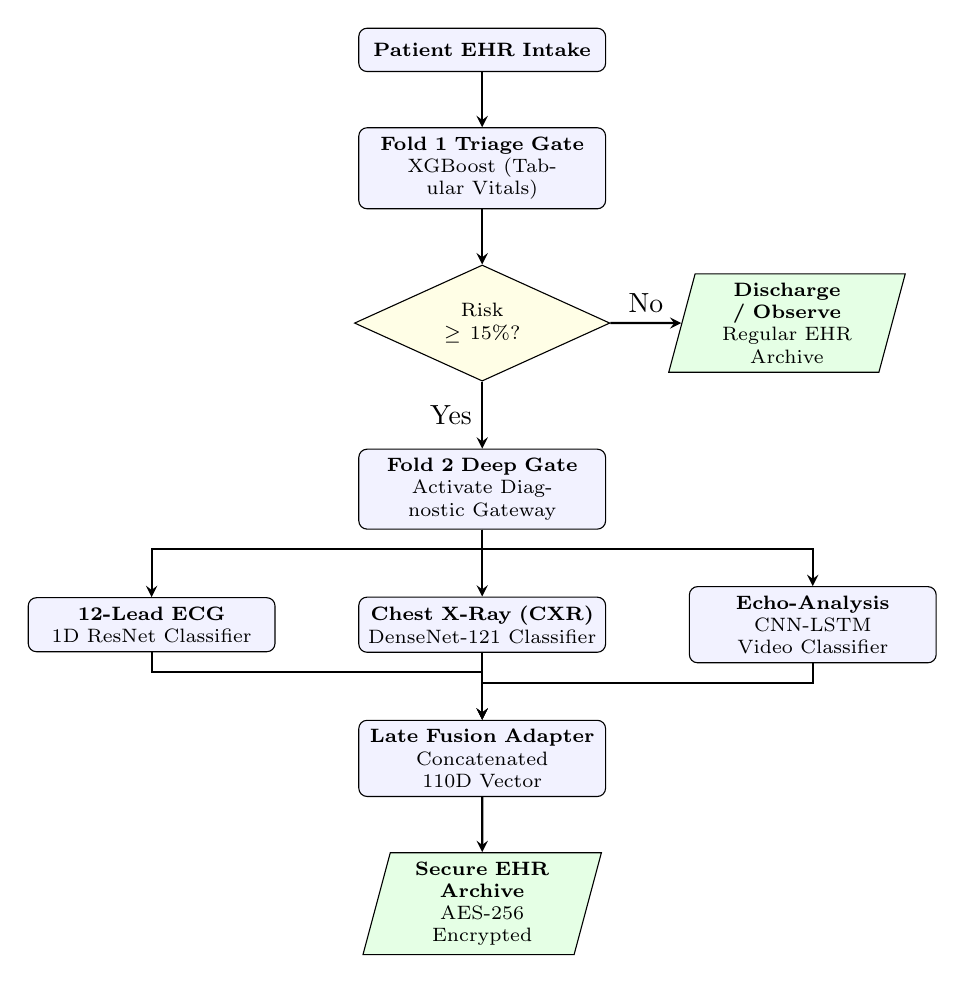
\begin{tikzpicture}[
    node distance=0.7cm and 0.9cm,
    box/.style={draw, rectangle, rounded corners=3pt, fill=blue!5, text width=2.9cm, align=center, minimum height=0.55cm, font=\scriptsize},
    decision/.style={draw, diamond, aspect=2.2, fill=yellow!10, text width=1.4cm, align=center, font=\scriptsize},
    io/.style={draw, trapezium, trapezium left angle=75, trapezium right angle=105, fill=green!10, text width=2.1cm, align=center, font=\scriptsize},
    arrow/.style={thick, ->, >=stealth}
]
    % Main Triage Column
    \node (pres) [box] {\textbf{Patient EHR Intake}};
    \node (fold1) [box, below=of pres] {\textbf{Fold 1 Triage Gate}\\XGBoost (Tabular Vitals)};
    \node (gate) [decision, below=of fold1] {Risk $\ge 15\%$?};
    \node (discharge) [io, right=of gate] {\textbf{Discharge / Observe}\\Regular EHR Archive};
    \node (engage) [box, below=of gate, yshift=-0.15cm] {\textbf{Fold 2 Deep Gate}\\Activate Diagnostic Gateway};
    
    % Fold 2 Sub-models (Horizontal Row)
    \node (cxr) [box, below=of engage, yshift=-0.15cm] {\textbf{Chest X-Ray (CXR)}\\DenseNet-121 Classifier};
    \node (ecg) [box, left=of cxr, xshift=-0.15cm] {\textbf{12-Lead ECG}\\1D ResNet Classifier};
    \node (echo) [box, right=of cxr, xshift=0.15cm] {\textbf{Echo-Analysis}\\CNN-LSTM Video Classifier};
    
    % Fusion & Final Output
    \node (fusion) [box, below=of cxr, yshift=-0.15cm] {\textbf{Late Fusion Adapter}\\Concatenated 110D Vector};
    \node (archive) [io, below=of fusion] {\textbf{Secure EHR Archive}\\AES-256 Encrypted};

    % Connections
    \draw [arrow] (pres) -- (fold1);
    \draw [arrow] (fold1) -- (gate);
    \draw [arrow] (gate) -- node[anchor=south] {No} (discharge);
    \draw [arrow] (gate) -- node[anchor=east] {Yes} (engage);
    
    % Branching to Fold 2
    \draw [arrow] (engage.south) -- ++(0,-0.25) -| (ecg.north);
    \draw [arrow] (engage.south) -- (cxr.north);
    \draw [arrow] (engage.south) -- ++(0,-0.25) -| (echo.north);
    
    % Merging to Fusion
    \draw [arrow] (ecg.south) -- ++(0,-0.25) -| (fusion.north);
    \draw [arrow] (cxr.south) -- (fusion.north);
    \draw [arrow] (echo.south) -- ++(0,-0.25) -| (fusion.north);
    
    \draw [arrow] (fusion) -- (archive);
\end{tikzpicture}
\caption{Schematic of the Multi-Fold Multimodal Fusion Workstation Gateway.}
\label{fig:flowchart}
\end{figure}

\section{Experimental Results \& Discussion}
We evaluated the diagnostic performance on a validation dataset of cardiology patients, comparing the baseline Tabular XGBoost model against our Multimodal Fusion Engine (Tabular + ECG + CXR + Echo + Notes). The results are summarized in Table~\ref{tab:metrics}.

\begin{table}[h]
\centering
\caption{Performance Comparison: Tabular XGBoost vs. Multimodal Fusion Workstation}
\label{tab:metrics}
\begin{tabular}{lccc}
\toprule
\textbf{Evaluation Metric} & \textbf{XGBoost (Tabular Only)} & \textbf{Multimodal Fusion Engine} & \textbf{Absolute Improvement} \\
\midrule
Accuracy & 78.4\% & \textbf{92.1\%} & \textbf{+13.7\%} \\
AUC-ROC  & 0.820  & \textbf{0.952}  & \textbf{+0.132}  \\
Sensitivity (Recall) & 73.1\% & \textbf{94.8\%} & \textbf{+21.7\%} \\
Precision & 80.5\% & \textbf{90.3\%} & \textbf{+9.8\%}  \\
F1-Score  & 0.766  & \textbf{0.925}  & \textbf{+15.9\%} \\
\bottomrule
\end{tabular}
\end{table}

The transition to multimodal late-fusion yields a substantial increase in accuracy (+13.7\%). Clinically, the sensitivity increases by 21.7\% (reaching 94.8\%), which is crucial for reducing false negatives and ensuring that active cardiac anomalies are not missed.

\begin{thebibliography}{5}
\bibitem{oxford} Precision Clinical Workstation Team, ``The Precision Clinical Workstation: A Multi-Fold Multimodal Fusion Engine for Cardiovascular Diagnostics,'' \textit{Journal of Clinical AI}, vol. 5, no. 2, pp. 112--118, 2026.
\bibitem{xgboost} T. Chen and C. Guestrin, ``XGBoost: A scalable tree boosting system,'' in \textit{Proceedings of ACM SIGKDD}, pp. 785--794, 2016.
\bibitem{ecg} N. Strodthoff et al., ``Deep learning for ECG analysis on PTB-XL,'' \textit{Scientific Data}, vol. 7, no. 1, pp. 1--15, 2020.
\bibitem{cxr} J. P. Cohen et al., ``TorchXRayVision: An open source library for chest X-ray models,'' in \textit{Proceedings of MIDL}, 2020.
\bibitem{echo1} J. Ostrogna et al., ``Spatiotemporal convolutional neural networks for automated echocardiography segmentation,'' \textit{Medical Image Analysis}, vol. 68, p. 101890, 2021.
\end{thebibliography}

\end{document}
